\section{Theory}

Franck and Hertz conducted a pioneering experiment in 1914 that offered the first tangible proof of quantized energy levels in atoms. They bombarded mercury vapor with electrons of varying energies and found a significant threshold: electrons with less than 4.9 electron volts (eV) could only undergo elastic collisions, whereas those with 4.9 eV or more could excite mercury atoms, resulting in the emission of light at a specific wavelength (253.6 nm). This observation provided strong support for Bohr's quantum theory, which posited that electrons could only occupy certain discrete energy states within an atom.

In this experimental arrangement, the excitation of neon atoms is investigated by observing inelastic collisions between electrons and neon atoms within a tetrode filled with neon gas. As electrons, emitted from a heated cathode and accelerated by an applied electric field, collide with neon atoms, the excited atoms release visible light. To determine the excitation energy of neon, the distance between the equidistant maxima of the electron current is measured under varying opposing electric fields. This analysis allows for a precise calculation of the energy required to excite neon atoms.

\subsection*{Principle}

Electrons are emitted from the cathode and accelerated towards the grid by applying a potential difference $U_{KG}$ between the cathode and the grid.The cathode in the tube is heated by a filament to emit electrons in a process called thermionic emission with an appplied voltage of $U_F$.

When electrons with insufficient energy (less than the excitation energy of the gas atoms) collide with the gas atoms, they do not transfer energy to the atoms. The collisions are elastic, meaning the electrons merely bounce off without losing kinetic energy.

When the electron energy equals or exceeds the excitation energy of the gas atoms, the electrons can transfer part of their energy to the atoms. This energy transfer
causes the atom to move from its ground state to an excited state. The energy required to excite the atom is quantized,

\begin{align}
    E_\text{exc} = \frac{hc}{\lambda} = eV
\end{align}

\subsection*{Excitation of Ne Atoms}
The most likely excitation in neon occurs when electrons collide inelastically, promoting atoms from the ground state to the ten $3p$ states, which are 18.4 to 19.0 eV above the ground state. The four lower $3s$ states, between 16.6 and 16.9 eV, are less likely to be excited. De-excitation from the $3p$ states back to the ground state happens through the $3s$ states, emitting photons in the process. The emitted light, visible to the naked eye, falls within the red to green range.

\begin{figure}[H]
    \centering
    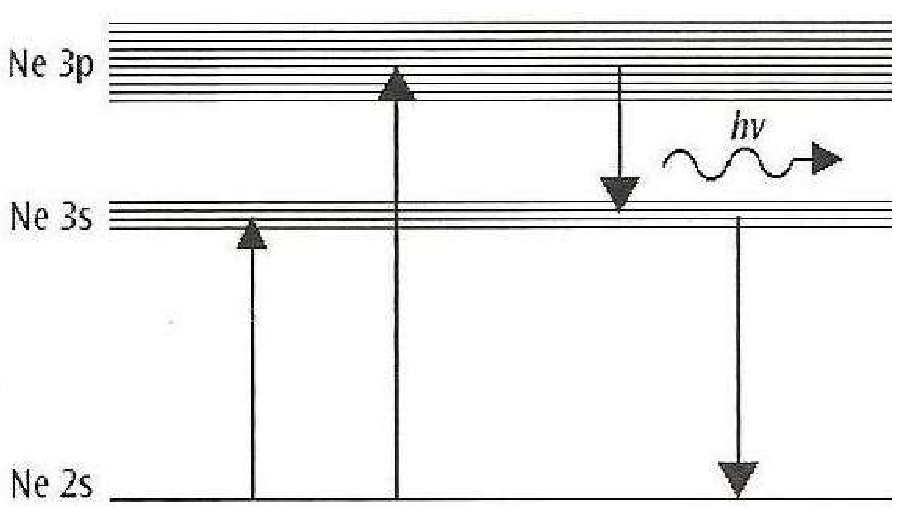
\includegraphics[width=0.8\columnwidth]{images/f1.png}
    \caption{Energy level diagram for Ne}
\end{figure}

% ==========================================================================
\section{Experimental Setup}

\subsection*{Apparatus}

\begin{enumerate}
    \item Franck-Hertz tube
    \item Franck-Hetrz Operating Unit
    \item Banana wires for connecting sockets for the heater, control grid and anode grid voltages\\
\end{enumerate}

Electrons are accelerated from the cathode (K) to the anode (A) by the applied voltage, denoted as $U_A$. A retarding potential, $U_{AE}$, is established between the anode (A) and the collector electrode (E), allowing only those electrons with sufficient kinetic energy to reach electrode E and contribute to the collector current.

\begin{figure}[H]
    \centering
    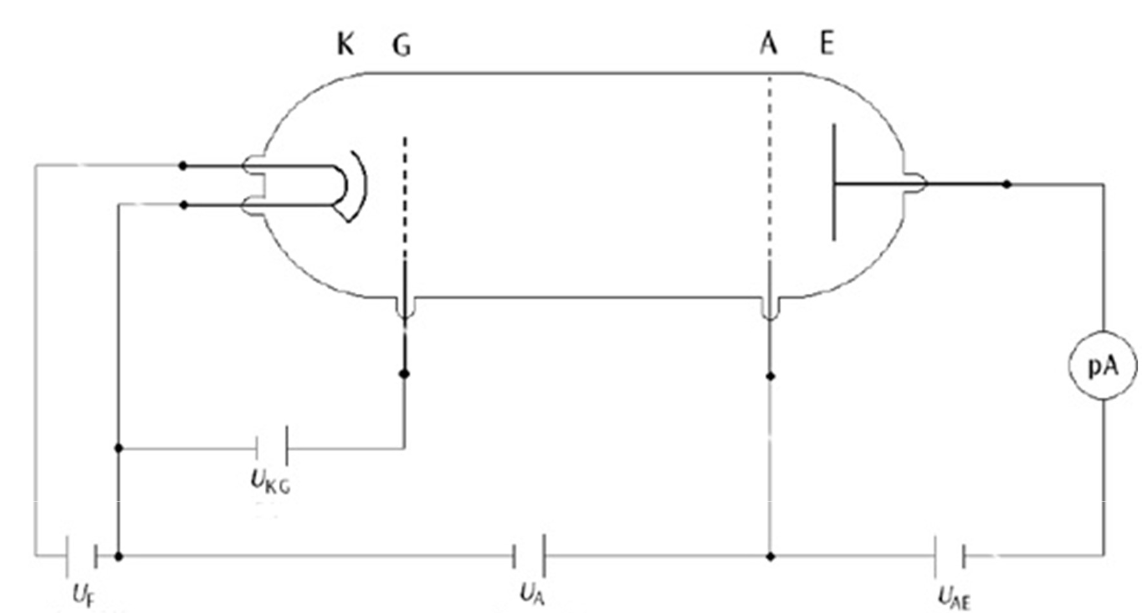
\includegraphics[width=1\columnwidth]{images/f2.png}
    \caption{Schematic of the experimental set-up and circuit diagram. Here, K is the cathode, G is the control grid, A is the anode and E is the collector electrode}
\end{figure}

As the accelerating voltage $U_A$ increases, the kinetic energy of the electrons rises. When this kinetic energy reaches the excitation energy of the gas atoms, inelastic collisions occur, causing electrons to lose energy and resulting in a decrease in the collected anode current. As $U_A$ continues to increase, electrons that have lost energy can be reaccelerated towards the anode. At even higher voltages, multiple inelastic collisions may occur, leading to a series of equidistant peaks and troughs in the anode current. By measuring the voltage difference between successive maxima in the anode current, the excitation energy of the gas can be determined,

\begin{align}
    E_\text{exc} = e\Delta U_A
\end{align}